%%%%%%%%%%%%%%%%%%%%%%%%%%%%%%%%%%%%%%%%%
% University/School Laboratory Report
% LaTeX Template
% Version 3.1 (25/3/14)
%
% This template has been downloaded from:
% http://www.LaTeXTemplates.com
%
% Original author:
% Linux and Unix Users Group at Virginia Tech Wiki 
% (https://vtluug.org/wiki/Example_LaTeX_chem_lab_report)
%
% License:
% CC BY-NC-SA 3.0 (http://creativecommons.org/licenses/by-nc-sa/3.0/)
%
%%%%%%%%%%%%%%%%%%%%%%%%%%%%%%%%%%%%%%%%%

%----------------------------------------------------------------------------------------
%	PACKAGES AND DOCUMENT CONFIGURATIONS
%----------------------------------------------------------------------------------------

\documentclass{article}

\usepackage{graphicx} % Required for the inclusion of images
\usepackage{amsmath} % Required for some math elements 
\usepackage{cite}
\usepackage{subcaption} %Required to group figures
\usepackage{float}

\setlength\parindent{0pt} % Removes all indentation from paragraphs

%\usepackage{times} % Uncomment to use the Times New Roman font

%----------------------------------------------------------------------------------------
%	DOCUMENT INFORMATION
%----------------------------------------------------------------------------------------

\title{Lab 5\\ Baseband PAM\\ EE 445S} % Title

\author{Enoc Balderas\\
        \and
        Daniel Diamont\\} % Author name

\date{\today} % Date for the report

\begin{document}

\maketitle % Insert the title, author and date

\begin{center}
\begin{tabular}{l r}
Date Performed: & March 1, 2019 \\ % Date the experiment was performed
Instructor: & Professor Evans % Instructor/supervisor
\end{tabular}
\end{center}

% If you wish to include an abstract, uncomment the lines below
% \begin{abstract}
% Abstract text
% \end{abstract}

%----------------------------------------------------------------------------------------
%	SECTION 1
%----------------------------------------------------------------------------------------

\section{Introduction}

For this  lab we experimented with the FIR and IIR filter design process.
We started off by using MATLAB's fdatool to experiment with different filter designs, and to gain intuition about the rules of thumb for meeting filter specifications.
Additionally we plotted the filter magnitude and phase to verify that the specifications have been met.
Finally we used the filter coefficients generated from MATLAB to implement IIR and FIR filters in C on our DSP board.

\subsection{Pulse Shaping}

We experimented with both sample based processing and frame based processing.
Within our sample based implementation we tested the difference in speed between a linear buffer and a circular buffer.
We also compared our sample based circular buffer implementation to a frame based processing implementation and compared the tradeoffs between them.

\subsection{SCR}

We experimented with a direct form II implementation and also a cascade of second order biquads.
We compared the implementation complexity of both methods and the number of coefficients required for each.
For instance biquads are reusable logic blocks, but there is lots of programming overhead setting up the biquad implementation.

\subsection{Demodulation}


%----------------------------------------------------------------------------------------
%	SECTION 2
%----------------------------------------------------------------------------------------

\section{Methods}

\subsection{Linear and Circular buffering}

We designed a 30th order FIR filter in MATLAB and recorded its magnitude response for frequencies between 1 - 24 kHz.
After confirming the response in MATLAB we exported the filter coefficients to a C file for implementation on DSP board.
On the DSP board we tested the clock cycles spent with both linear and circular buffers.

\subsection{Frame based processing}

Using the same FIR filter coefficients we experimented with a frame based approach and compared the results to the circular buffer sample based implementation.
We also experimented with the compiler optomizations available in CCS for a convolution method written in C compared to one in assebly.

\subsection{IIR filtering}

We designed a 6th order IIR filter in MATLAB and recorded its magnitude response for frequencies between 1 - 24 kHz.
After confirming the response in MATLAB we exported the filter coefficients to a C file for implementation on DSP board.
We compared the performance of the direct form implementation with a second order biquad cascade.
 
%----------------------------------------------------------------------------------------
%	SECTION 3
%----------------------------------------------------------------------------------------

\section{Results}

\subsection{Pulse Shaping}

\begin{figure}[h]
  \begin{center}
    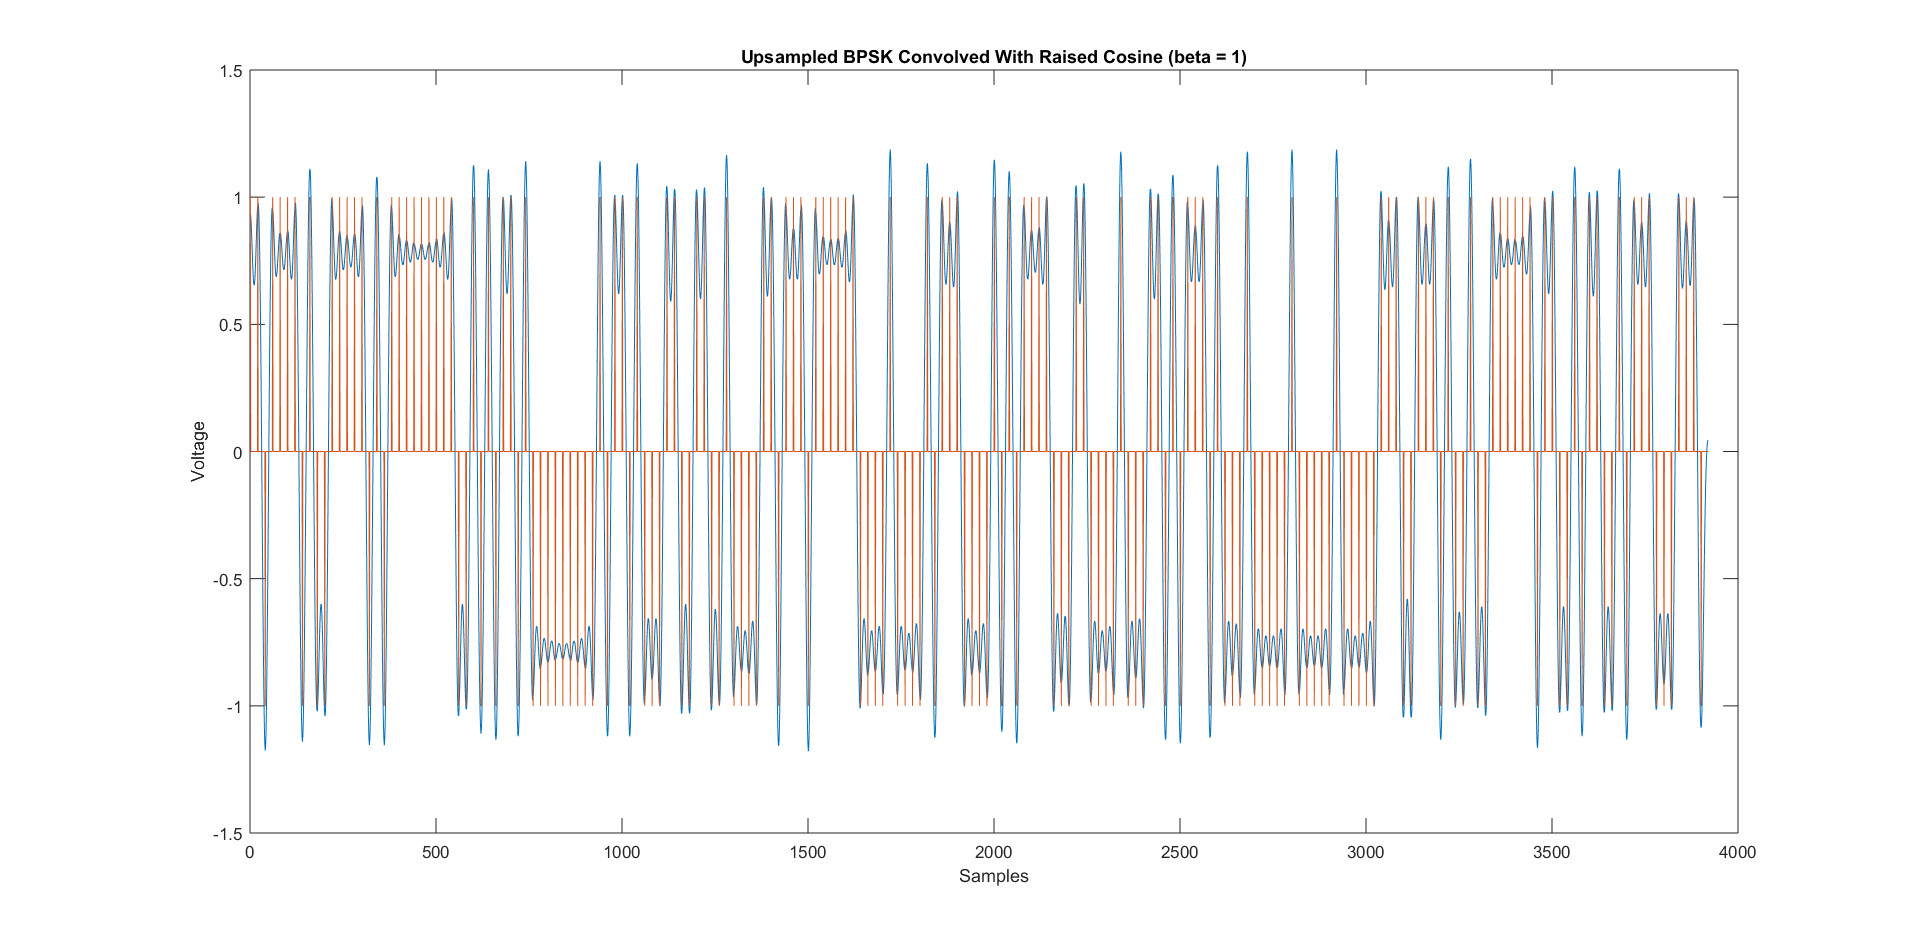
\includegraphics[width=0.65\textwidth]{img/upsampled_bpsk_raised_cosine_beta_1.png}
    \caption{Pulse shape BPSK $\beta = 1$.}
  \end{center}
\end{figure}

\begin{figure}[h]
  \begin{center}
    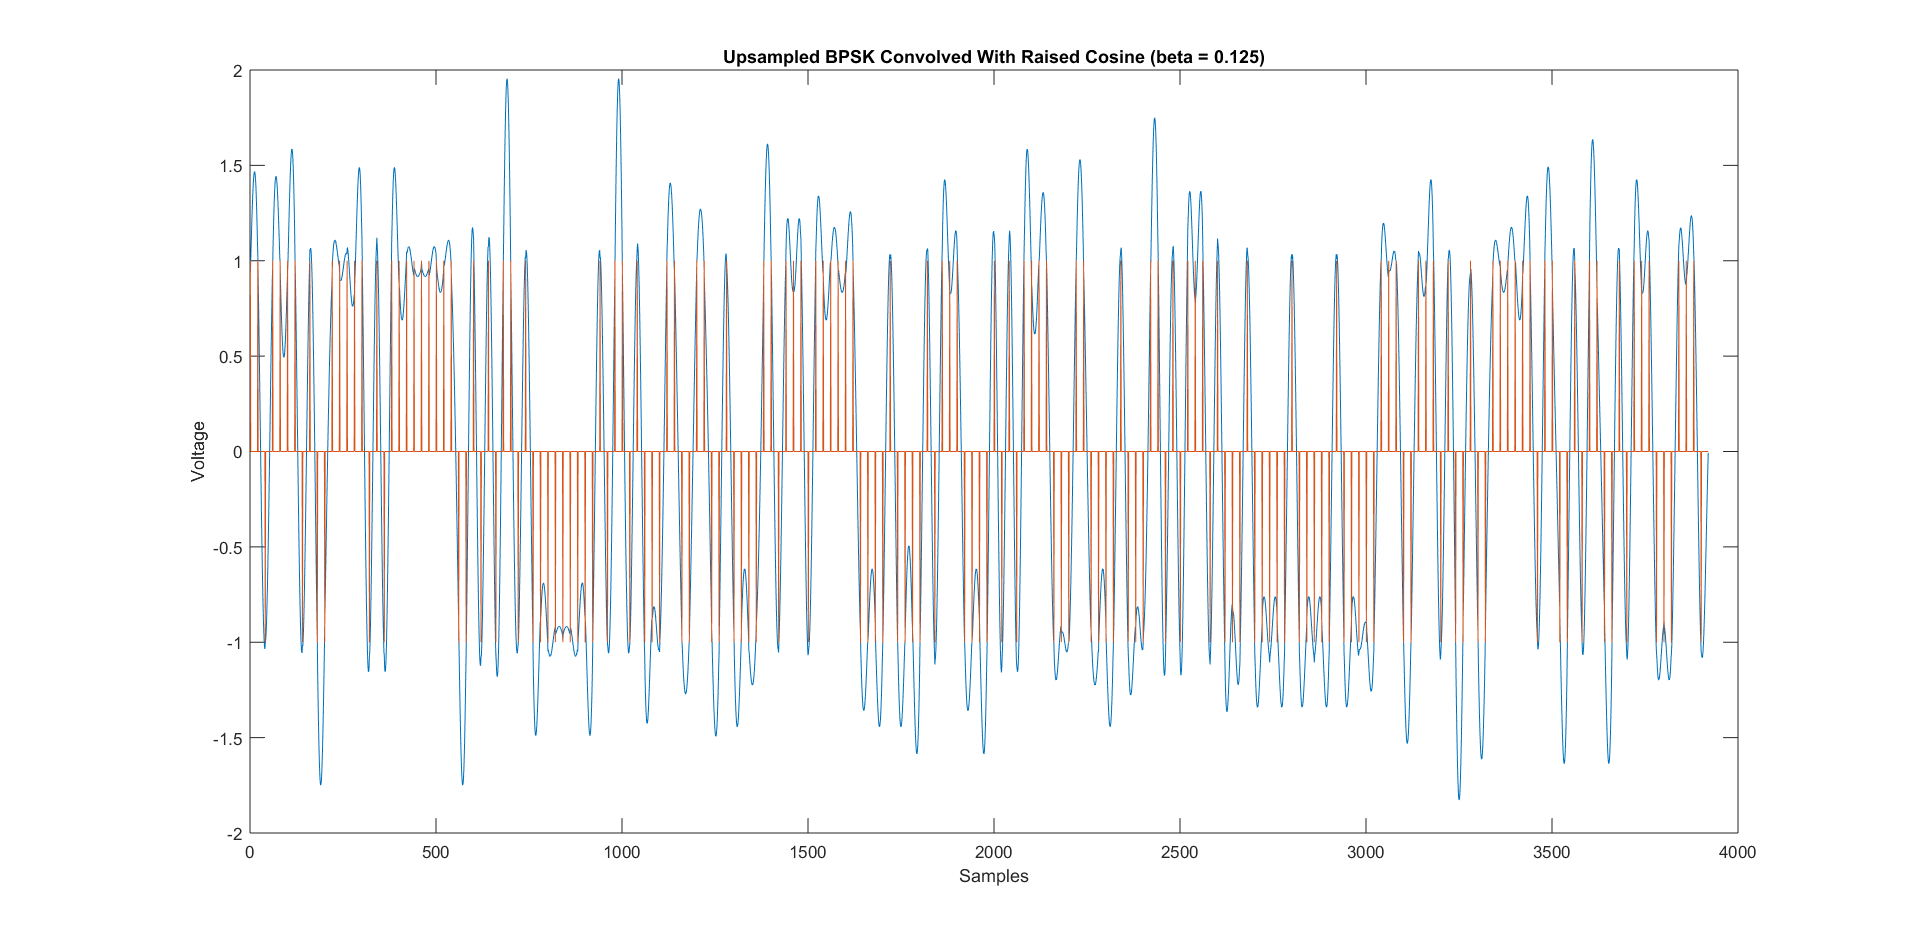
\includegraphics[width=0.65\textwidth]{img/upsampled_bpsk_raised_cosine_beta_125.png}
    \caption{Pulse shape BPSK $\beta = 0.125$.}
  \end{center}
\end{figure}

\begin{figure}[h]
  \begin{center}
    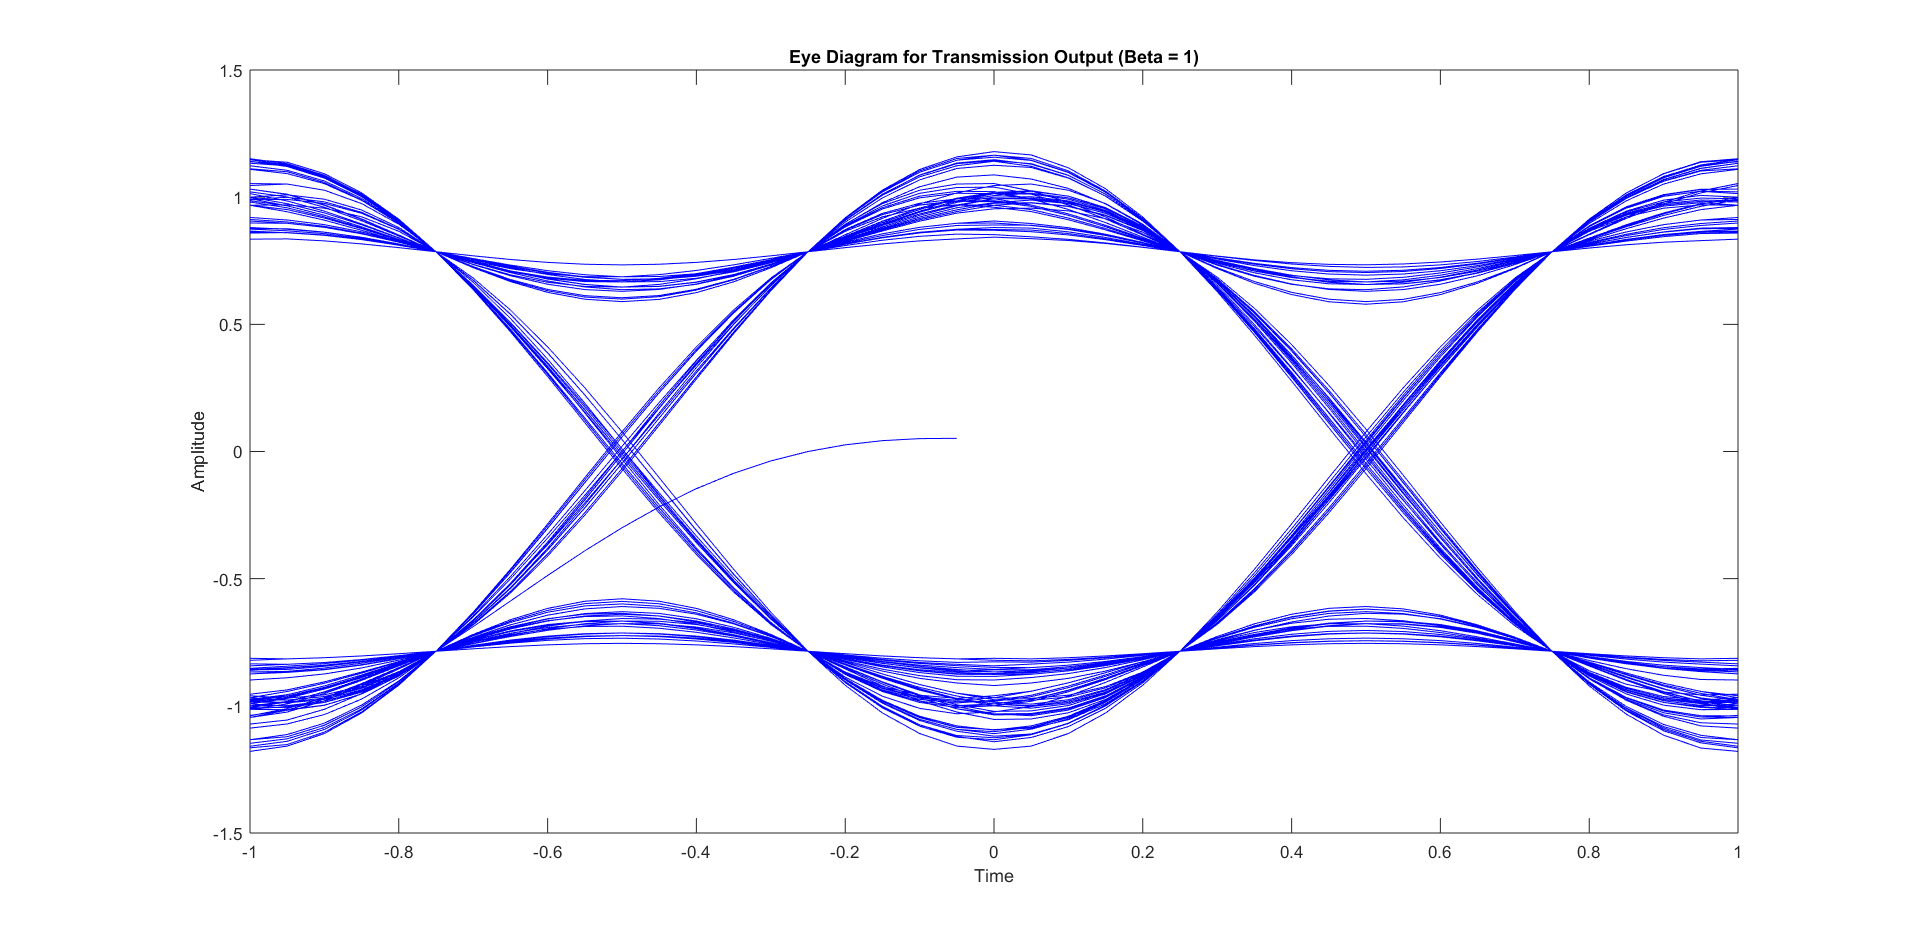
\includegraphics[width=0.65\textwidth]{img/eye_diagram_beta_1.png}
    \caption{Eye diagram $\beta = 1$}
  \end{center}
\end{figure}

\begin{figure}[h]
  \begin{center}
    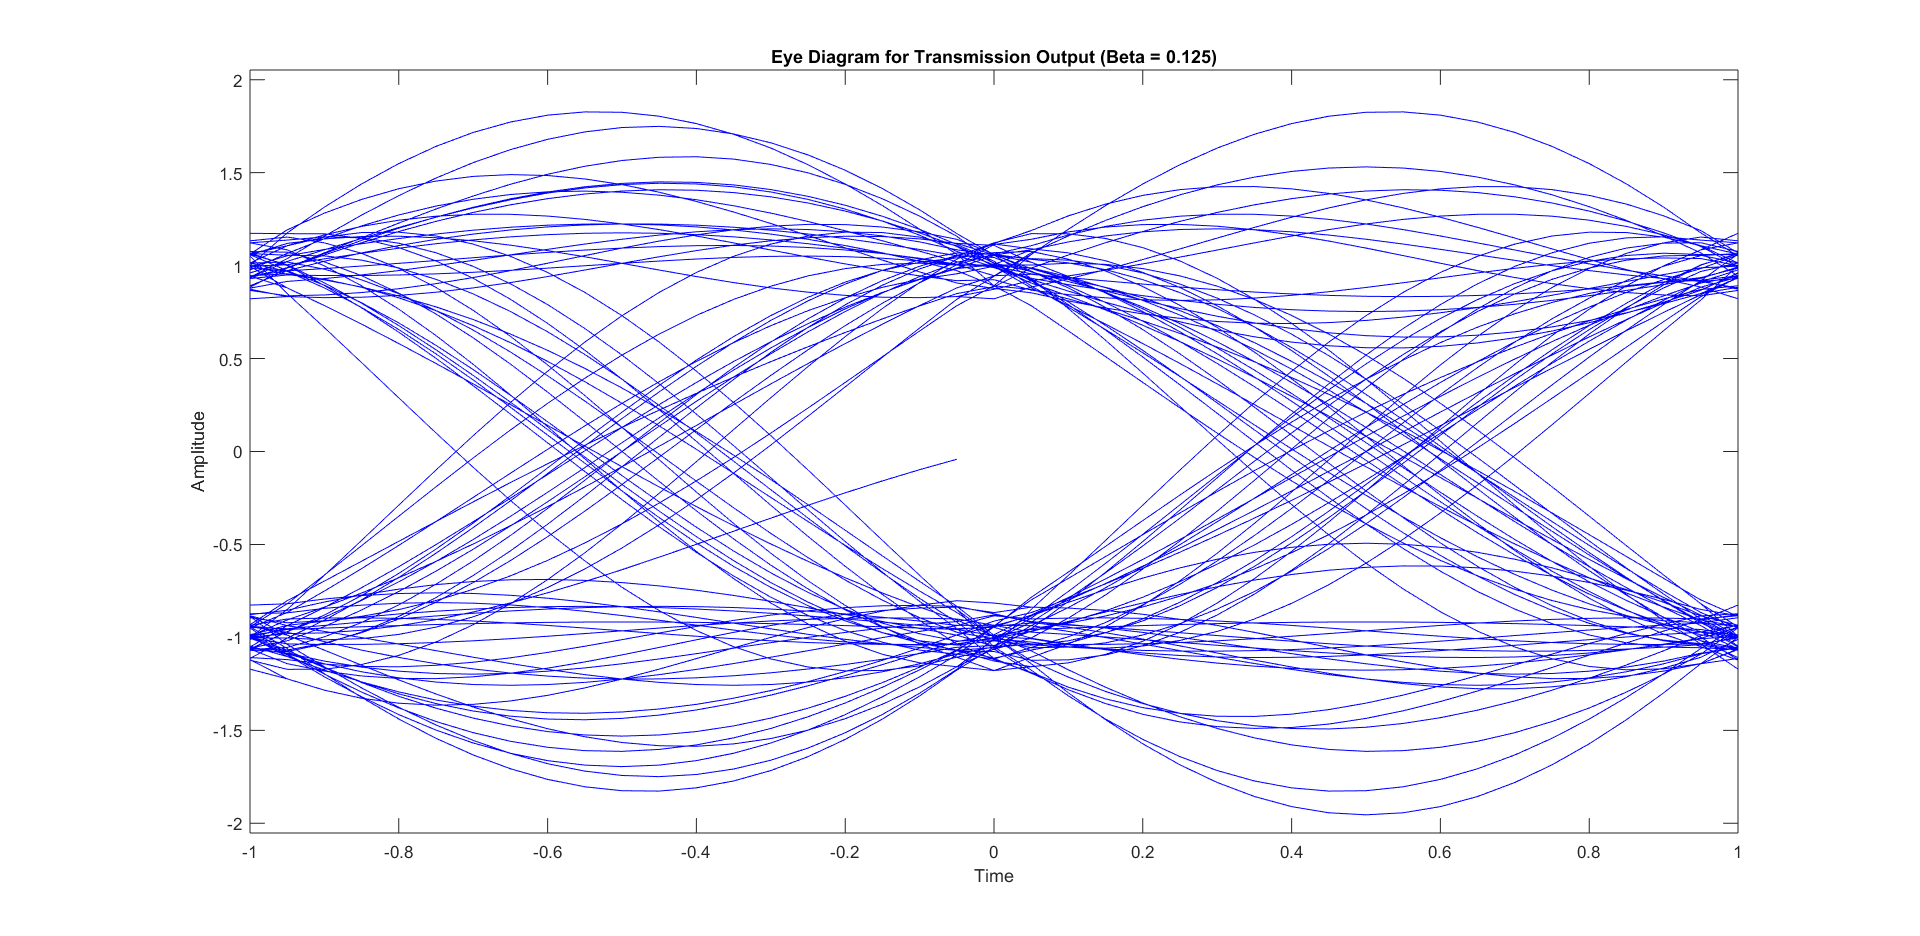
\includegraphics[width=0.65\textwidth]{img/eye_diagram_beta_125.png}
    \caption{Eye diagram $\beta = 0.125$}
  \end{center}
\end{figure}

\begin{figure}[h]
  \begin{center}

    \begin{subfigure}[b]{0.5\linewidth}
      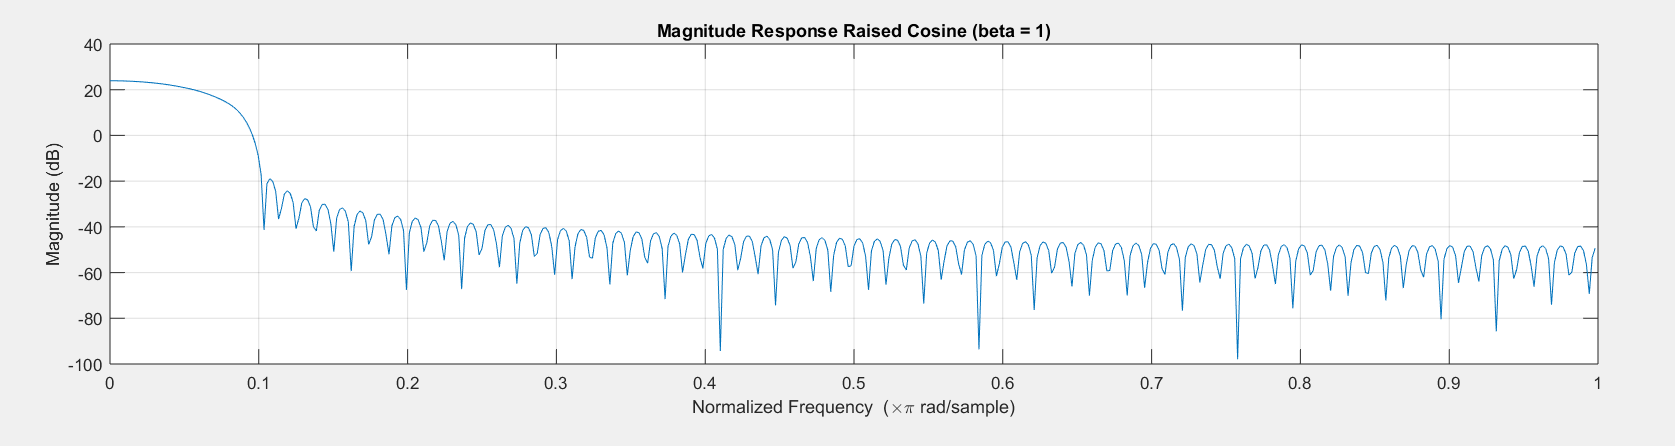
\includegraphics[width=\linewidth]{img/magnitude_response_beta_1.png}
      \caption{Magnitude Response $\beta = 1$}
    \end{subfigure}

    \begin{subfigure}[b]{0.5\linewidth}
      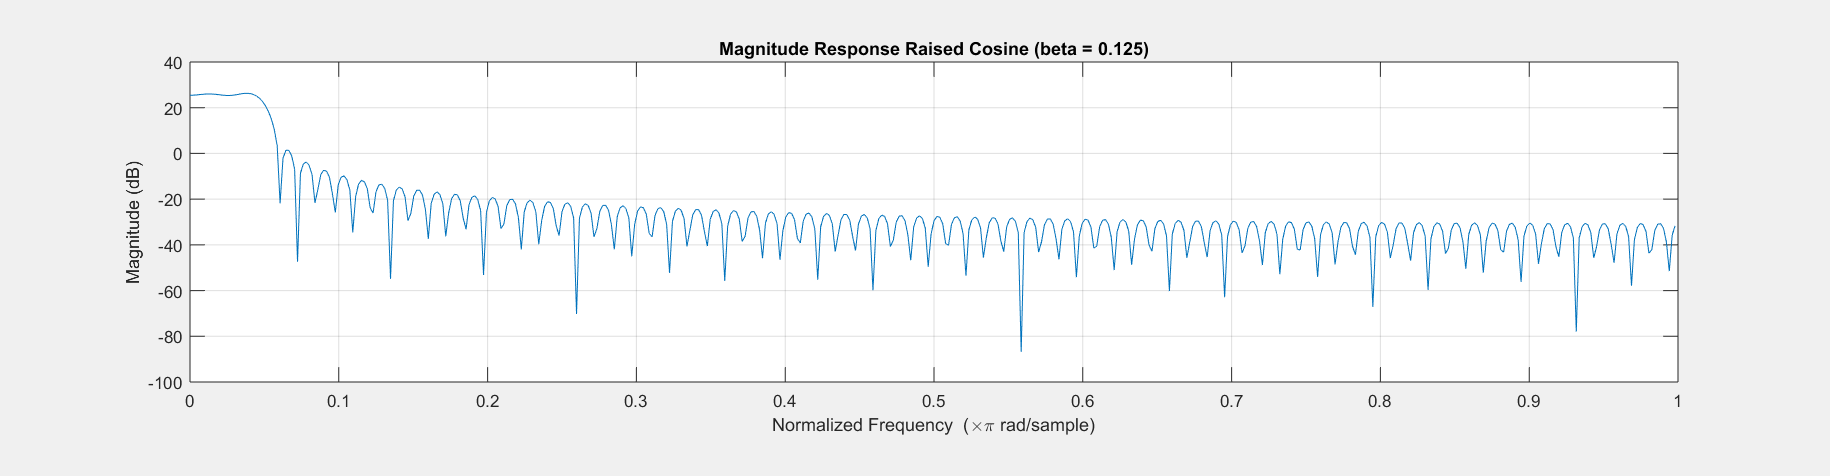
\includegraphics[width=\linewidth]{img/magnitude_response_beta_125.png}
      \caption{Magnitude Response $\beta = 0.125$}
    \end{subfigure}

  \end{center}
\end{figure}

\begin{figure}[h]
  \begin{center}

    \begin{subfigure}[b]{0.5\linewidth}
      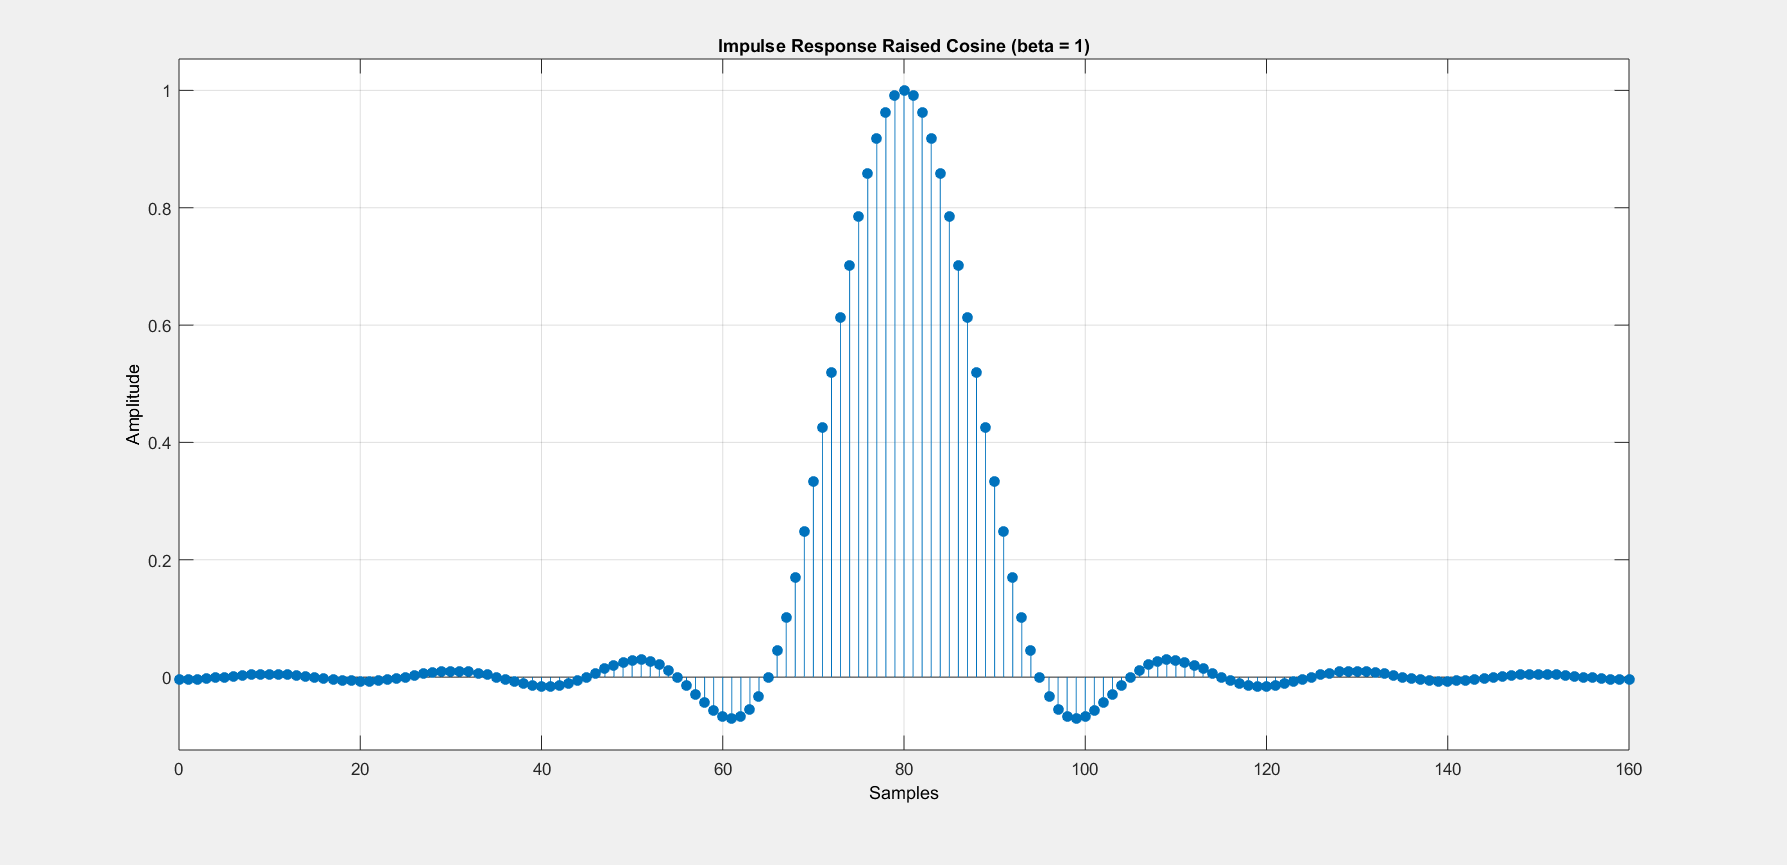
\includegraphics[width=\linewidth]{img/impulse_response_beta_1.png}
      \caption{Time Response $\beta = 1$}
    \end{subfigure}

    \begin{subfigure}[b]{0.5\linewidth}
      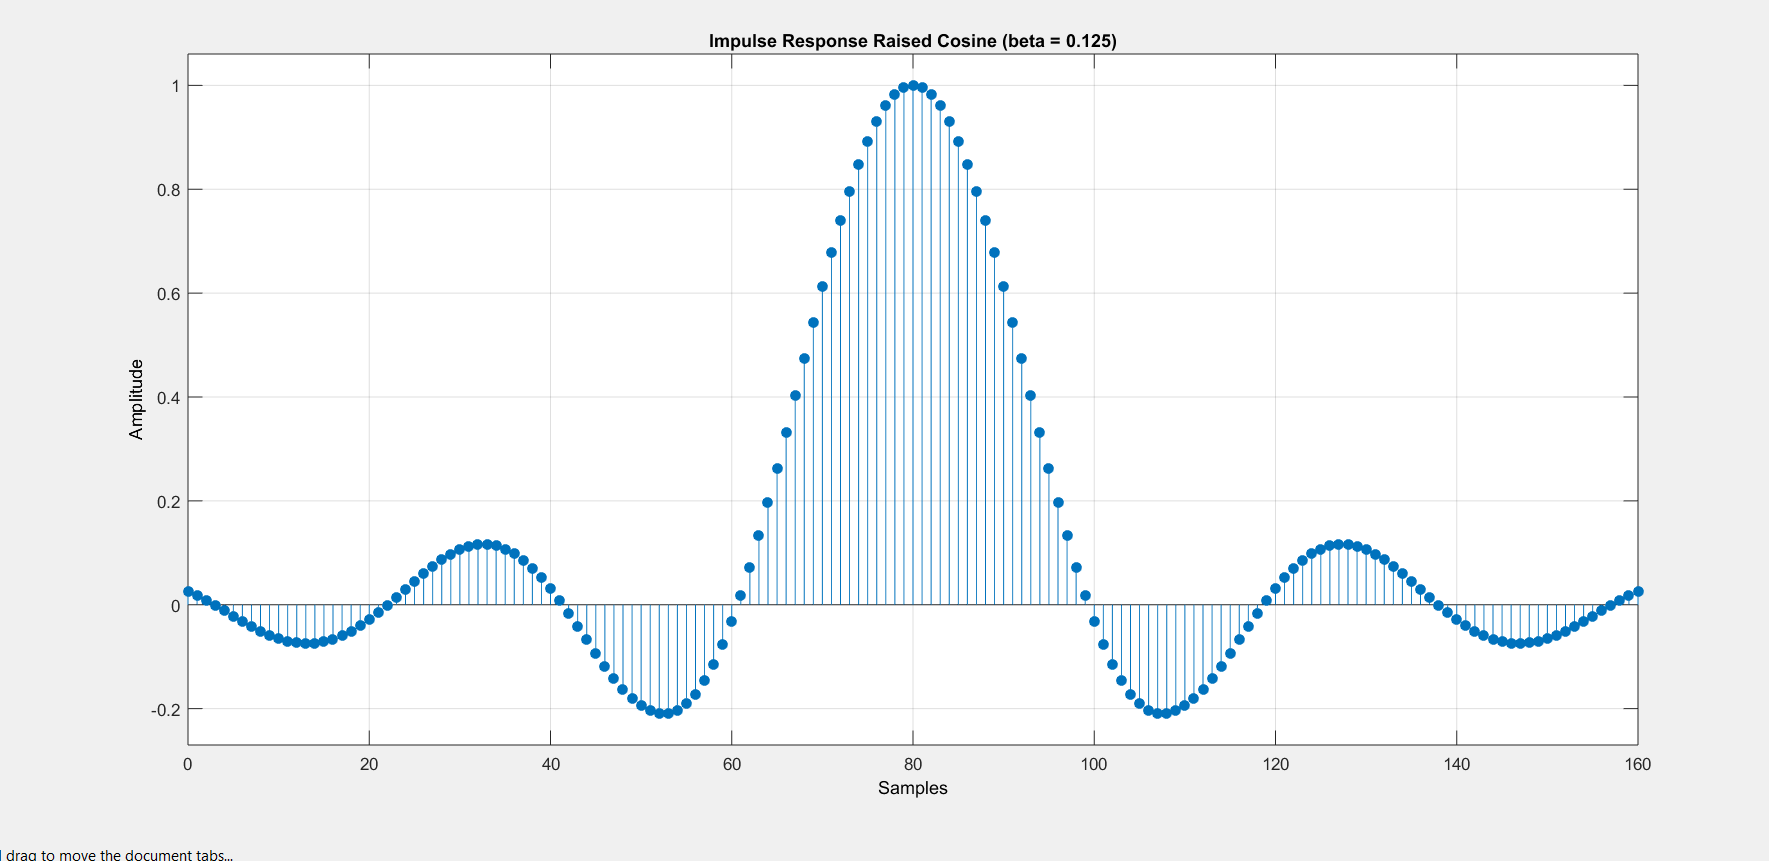
\includegraphics[width=\linewidth]{img/impulse_response_beta_125.png}
      \caption{Time Response $\beta = 0.125$}
    \end{subfigure}

  \end{center}
\end{figure}

\begin{enumerate}
  \begin{item}
  Explain the major differences between the two filters with respect to their
    A) Magnitude responses 
    B) Impulse responses

  \textbf{Answer:}
    A) The main difference between the magnitude response is that the $\beta = 0.125$ filter has
    a much lower bandwidth than the $\beta = 1$ filter.\\

    B) The main difference between the impulse response is that the $\beta = 0.125$ filter
    side lobes decay at a slower rate than the $\beta = 1$ filter side lobes.
  \end{item}

  \begin{item}
    What is the width of the impulse response for the $\beta = 0.125$ case? 

  \textbf{Answer:}
  \end{item}

  \begin{item}
    How would you obtain this number theoretically? (Hint: Look at the fsym and truncation limit you set)

  \textbf{Answer:}
  \end{item}

\end{enumerate}

\begin{figure}[h]
  \begin{center}

    \begin{subfigure}[b]{0.5\linewidth}
			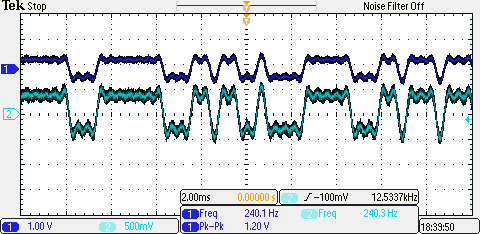
\includegraphics[width=0.65\textwidth]{img/DSK_implementation_beta_1.png}
      \caption{Time Response $\beta = 1$}
    \end{subfigure}

    \begin{subfigure}[b]{0.5\linewidth}
			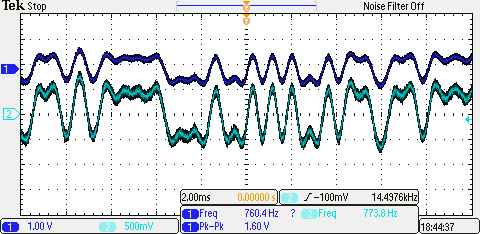
\includegraphics[width=0.65\textwidth]{img/DSK_implementation_beta_125.png}
      \caption{Time Response $\beta = 0.125$}
    \end{subfigure}

  \end{center}
\end{figure}

\subsection{Symbol Clock Recovery}

\textbf{Prefilter:}

\begin{center}
\begin{tabular}{c|c}
b0	&	 1				\\ \hline
b1	&  0				\\ \hline
b2	& -1				\\ \hline
-a1	&	 1.96004	\\ \hline
-a2	&	-0.984414
\end{tabular}
\end{center}

\textbf{Bandpass:}

\begin{center}
\begin{tabular}{c|c}
b0	&	 1				\\ \hline
b1	&  0				\\ \hline
b2	& -1				\\ \hline
-a1	&	 1.87293\\ \hline
-a2	&	-0.969067
\end{tabular}
\end{center}

\begin{figure}[h]
  \begin{center}
    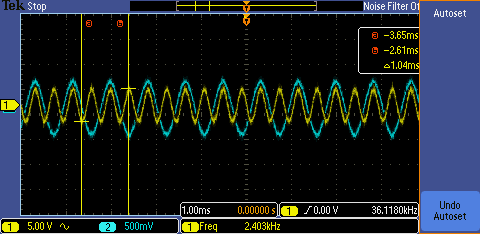
\includegraphics[width=0.65\textwidth]{img/dotting_sequence_SCR.png}
    \caption{Dotting sequence}
  \end{center}
\end{figure}

\begin{figure}[h]
  \begin{center}
    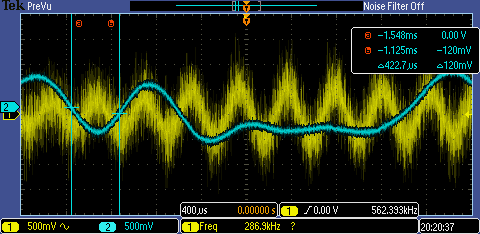
\includegraphics[width=0.65\textwidth]{img/2PAM_SCR.png}
    \caption{2-PAM SCR}
  \end{center}
\end{figure}

\pagebreak
\textbf{Code:}

\begin{verbatim}
	if (counter == 0) {
		symbol = SSRG_update(&SSRG_state); // pseudo random m-sequence
		x[0] = data[symbol]; // read the table

		/* dotting sequence
		symbol = symbol ^ 1;
		x[0] = data[symbol]; // read the table
		*/
	}

	// perform impulse modulation based on the FIR filter, B[N] 

	y  = 0;

	for (i = 0; i < 8; i++) {
		y +=  x[i]*B[counter + 20*i];	// perform the dot-product
	}

	if (counter == (samplesPerSymbol - 1)) {
		counter = -1; 

		/* shift x[] in preparation for the next symbol */

		for (i = 9; i > 0; i--) {
			x[i] = x[i - 1];          // setup x[] for the next input
		}
	}

	counter++;

	output = y;
	scr = clock_recover(y);
\end{verbatim}

\textbf{Table:}

\begin{center}
\begin{tabular}{c|c|c}
pattern	&	frequency & amplitude \\ \hline
dotted sequence	&	 2381 Hz	&	1.04 V				\\ \hline
dotted sequence	&	 2323 Hz	&	1.46 V
\end{tabular}
\end{center}

\textbf{LPF:}

\begin{center}
\begin{tabular}{c|c}
b0	&	 1				\\ \hline
b1	&  1				\\ \hline
b2	&  0				\\ \hline
-a1	&	 0.509525\\ \hline
-a2	&	 0
\end{tabular}
\end{center}

\textbf{Code:}

\begin{verbatim}
  if (counter == 0) {
		symbol = SSRG_update(&SSRG_state); // a faster version of rand() % 2
		x[0] = data[symbol]; // read the table
	}

  // perform impulse modulation based on the FIR filter, B[N] 
  y  = 0;

  for (i = 0; i < 8; i++) {
		y +=  x[i]*B[counter + 20*i];	// perform the dot-product
	}

  if (counter == (samplesPerSymbol - 1)) {
    counter = -1; 

		/* shift x[] in preparation for the next symbol */
 		for (i = 9; i > 0; i--) {
			x[i] = x[i - 1];          // setup x[] for the next input
		}
  }

  counter++;

	output = y*cosine[counter & 3];

	//receiver
	demod = 2*output*cosine[counter & 3];

	//LPF
	biquad_x[0][0] = demod;

	CodecDataOut.Channel[LEFT]  = y; // setup the LEFT  value
	CodecDataOut.Channel[RIGHT] = G[0] * biquad(0, biquad_x[0][0]); // setup the RIGHT value
\end{verbatim}

\begin{figure}[h]
  \begin{center}
    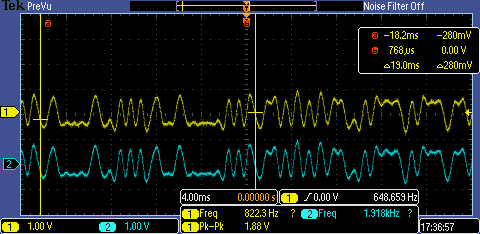
\includegraphics[width=0.65\textwidth]{img/tx_rx.png}
    \caption{transmit and recieve}
  \end{center}
\end{figure}

\begin{figure}[h]
  \begin{center}
    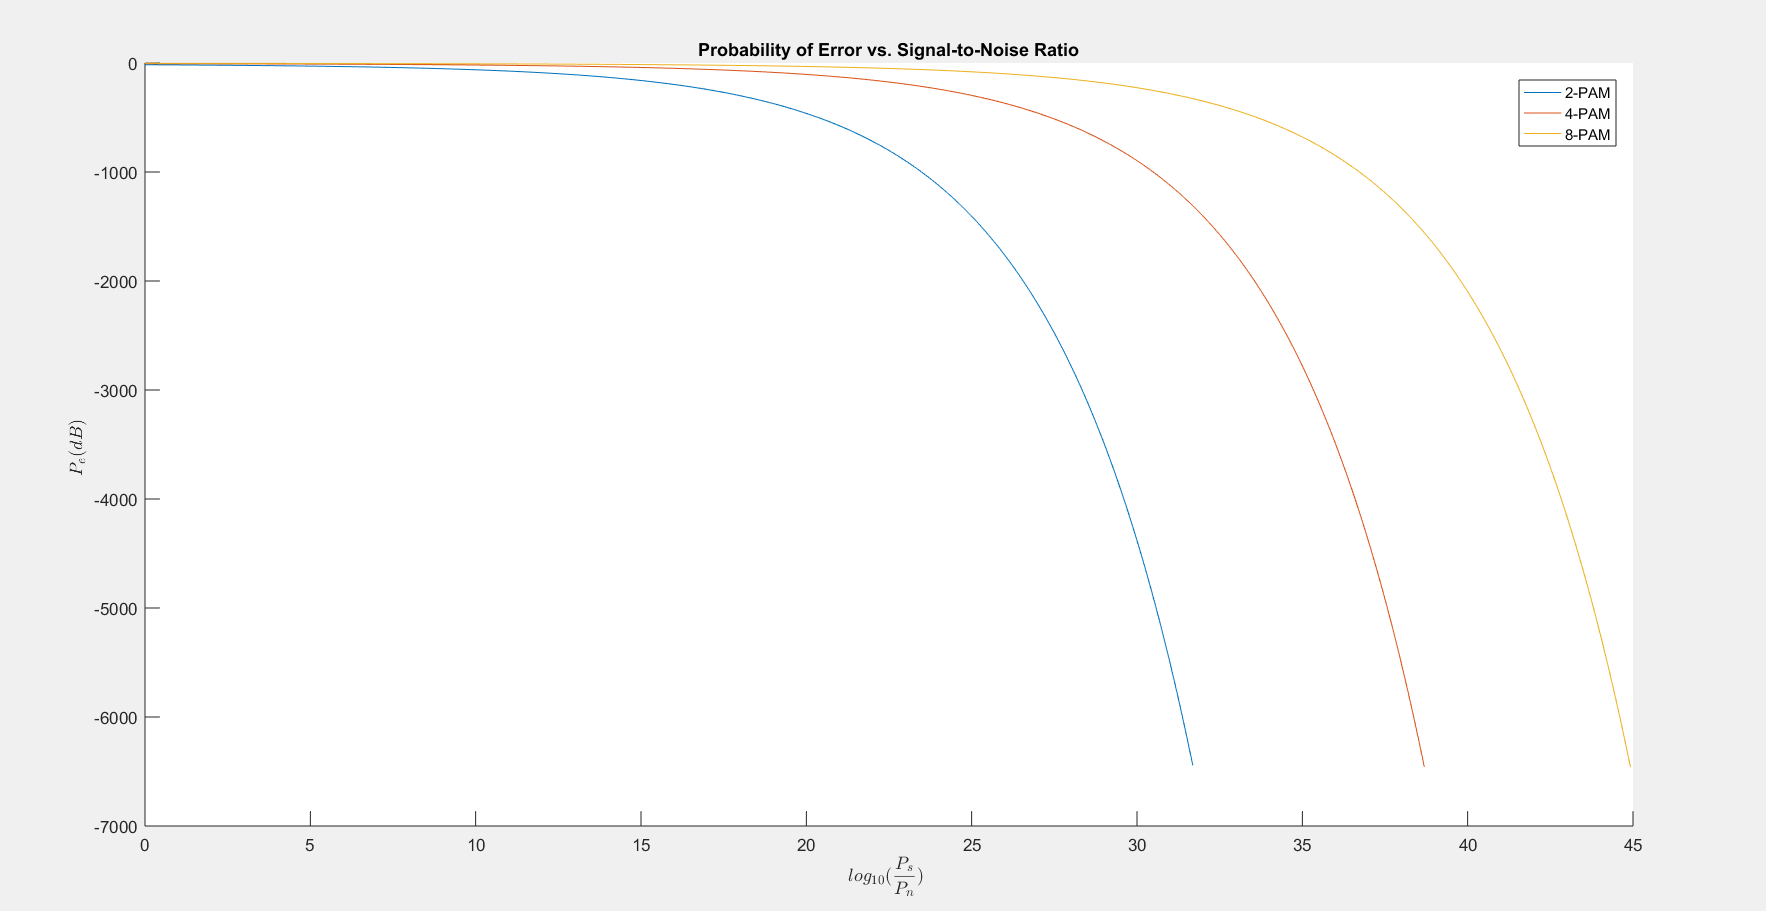
\includegraphics[width=0.65\textwidth]{img/probability_of_error.png}
    \caption{PES}
  \end{center}
\end{figure}

%----------------------------------------------------------------------------------------
%	SECTION 4
%----------------------------------------------------------------------------------------

\section{Discussion}

\subsection{Linear and Circular buffering}

We learned that the MATLAB fda tool is very good for quickly designing filters.
After examining the magnitude plot in MATLAB we got a good idea about what to expect from the real time implementation.

\subsection{Frame based processing}

One big take away was that the compiler is a way better optimizer than we are.
Also we realized that some compiler optimizations lead to very hard to understand assembly code.

\subsection{IIR filtering}

It was a surprise that the IIR filter achieved such great performance with far less filter coefficients.
Also it was interesting to see the effect of using incorrect gains in the cascuade of biquads.

%----------------------------------------------------------------------------------------
%	SECTION 5
%----------------------------------------------------------------------------------------

\section{Answers to questions}

\begin{enumerate}
  \begin{item}
		How could pulse shaping be implemented using only a single "filter" (not a bank of filters). Practically, why would this be undesirable?

  \textbf{Answer:}
		Pulse shaping could be implemented by convolving with a single FIR filter. This is undesirable because for baseband transmission we usually take our symbol amplitude vector and upsample (by some fator L) to the DAC frequency before pulse shaping. Because of this upsampling, the amplitude vector contains a lot of extra zeros, which would cause (L - 1) multiplications by 0 for every original symbol amplitude. By using a filter bank, we avoid these
		fruitless multiplications by 0, and obtain a factor of L performance improvement.
  \end{item}

  \begin{item}
		In the clock recovery system, discuss the need for a Prefiltering. For a symbol rate of 2 kHz, what would be the output if the prefilter attenuated all frequencies greater than 900 Hz? Would it be possible to recover the transmitter's symbol frequency (using the same squaring operation and post-filters as in the lab)? If not, give a short reason why.

  \textbf{Answer:}
		We prefilter to obtain a cosine with a center frequency of $fsym/2$ without high frequency noise. What we are interested in is capturing the phase ($\theta$) and frequency information (fsym) of the cosine to feed this into a Costas or Phase Lock Loop to determine the phase offset for sampling. Any other frequency content is unnecessary.

		If the output of the prefilter attenuated all frequencies greater than 900 Hz, we would not be able to recover the transmitter's symbol frequency because $fsym/2$ in this case equals 1 KHz, which would be attenuated by our hypothetical prefilter.
  \end{item}

\end{enumerate}

%----------------------------------------------------------------------------------------
%	BIBLIOGRAPHY
%----------------------------------------------------------------------------------------

\bibliography{mybib}
\bibliographystyle{plain}

%----------------------------------------------------------------------------------------


\end{document}
